\documentclass{beamer}
\usepackage{HECbeamer}
\usepackage{icomma}
% \usepackage{pgfpages}
% \pgfpagesuselayout{4 on 1}[letterpaper, landscape, border shrink=5mm]
\title[\color{white}{MATH 60604 \S~4f - Surdispersion}]{\texorpdfstring{MATH 60604 \\Modélisation statistique \\ \S~4f - Surdispersion}{MATH 60604 \\Modélisation statistique \\ \S~4f - Surdispersion}}
\author{}
\institute{HEC Montréal\\
Département de sciences de la décision}
\date{} 

\begin{document}
\frame{\titlepage}

\begin{frame}[fragile]
\frametitle{Extension du modèle de Poisson et surdispersion}
\bi
\item La loi de Poisson n'est pas très flexible car elle possède un seul paramètre qui régule à la fois sa moyenne et sa variance.
\item Dans plusieurs cas, cette hypothèse n'est pas valide. Dans l'exemple d'intention d'achat, le rapport déviance sur degrés de liberté était  $203,27/110 = 1,85$, ce qui suggérait que le modèle de Poisson ajusté n'était \textbf{pas adéquat} (valeur-$p$ inférieure à $10^{-5}$).
\item Une des raisons sous-jacentes pour cette piètre performance est la surdispersion, lorsque la variabilité des données de dénombrement est plus élevée que leur moyenne.
\item La modèle de régression \alert{binomiale négative} est souvent utilisé dans ces cas de figure.
\ei
\end{frame}


\begin{frame}[fragile]
\frametitle{Loi binomiale négative}
\bi
\item La loi  binomiale négative est une loi de probabilité pour une variable  \alert{entière} dotée de deux paramètres.
\item On considère la paramétrisation la plus courante pour la modélisation. La fonction de masse est
\begin{align*}
\P{Y=y}=\frac{\Gamma(y+1/k)}{\Gamma(y+1)\Gamma(1/k)} \left(\frac{1/k}{1/k + \mu} \right)^{1/k} \left(\frac{\mu}{1/k+\mu}\right)^y
\end{align*}
pour $y=0, 1, 2, 3, \ldots$, où $\Gamma$ dénote la fonction gamma. Les deux paramètres de la loi sont positifs, $\mu>0$ et $k>0$.

\item La moyenne théorique et la variance sont \begin{align*}
\E{Y}=\mu, \qquad \Va{Y}=\mu+k\mu^2.                                 \end{align*}
\item La variance d'une variable binomiale négative est donc \alert{supérieure} à sa moyenne. 
\ei
\end{frame}


\begin{frame}[fragile]
\frametitle{Régression binomiale négative}
\bi
\item Dans la régression binomiale négative, on postule que la variable réponse $Y$ 
suit une loi \alert{binomiale négative} avec \alert{fonction de liaison} logarithmique
\begin{align*}
g\{\E{Y_i}\}=\ln\{\E{Y_i}\}=\beta_0+\beta_1\mathrm{X}_{i1}+\ldots+\beta_p\mathrm{X}_{ip}.
\end{align*}
\item De manière équivalente, cela revient à assumer que la $i$e observation, $Y_i$, suit une loi binomiale négative de moyenne
\begin{align*}
\E{Y_i}=\exp(\beta_0+\beta_1\mathrm{X}_{i1}+\ldots+\beta_p\mathrm{X}_{ip})
\end{align*}
\item Ainsi, l'interprétation des paramètres se fait de manière identique à la
régression de Poisson. 

\item En revanche, la régression binomiale négative a un autre paramètre, $k$. Ce dernier est supposé \alert{identique pour
chaque observation}. Il ne dépend donc pas des variables explicatives.
\ei

{ \tiny Tangente mathématique:
À proprement parler, la régression binomiale négative ne fait pas partie des modèles linéaires généralisés parce que cette loi fait partie de la famille de dispersion exponentielle. On peut ajuster le modèle par maximum de vraisemblance et la machinerie développée pour les GLM s'applique néanmoins.

}
\end{frame}



\begin{frame}[fragile]
\frametitle{Régression binomiale négative avec \code{proc genmod}}
La seule différence avec le modèle de Poisson est la loi des réponses, viz. \texttt{dist=negbin}. 
\begin{tcolorbox}[colback=white, colframe=hecblue, title=Code SAS code pour ajuster une régression binomiale négative]
% proc glimmix data=modstat.regdenombrement1;
% class educ revenu;
% model nombreachat=sexe age revenu educ statut 
%      fixation emotion / dist=negbin link=log solution;
% run;
\begin{verbatim}
proc genmod data=modstat.intention;
class educ revenu;
model nachat=sexe age revenu educ statut
     fixation emotion / dist=negbin link=log
     lrci type3;
run;
\end{verbatim}
\end{tcolorbox}
{\footnotesize 
Dans \Rlang, la paramétrisation de \texttt{MASS:glm.nb} est telle que $\theta=1/k$.

}
\end{frame}

\begin{frame}[fragile]
\frametitle{Qualité de l'ajustement pour le modèle binomiale négative}
\begin{center}
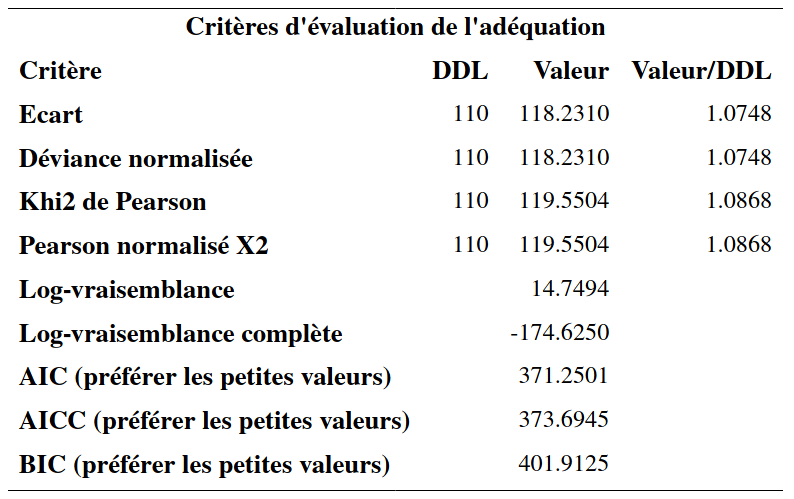
\includegraphics[width = 0.6\linewidth]{img/c4/diapos8-e6}
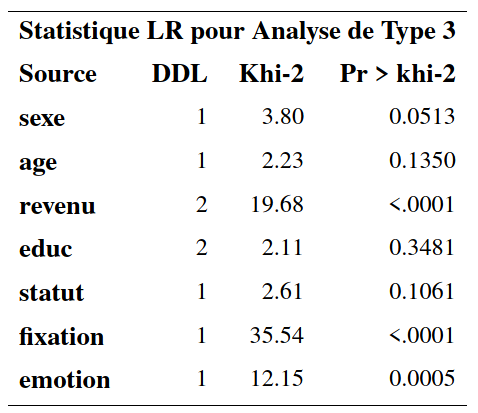
\includegraphics[width = 0.39\linewidth]{img/c4/diapos8-e7}
\end{center}
La déviance est plus près de un. À cause de l'inflation de la variance, seules les variables \texttt{revenu}, \texttt{fixation} et \texttt{emotion} sont significatives.
\end{frame}

\begin{frame}[fragile]
\frametitle{Estimés des paramètres pour la régression binomiale négative}
\begin{center}
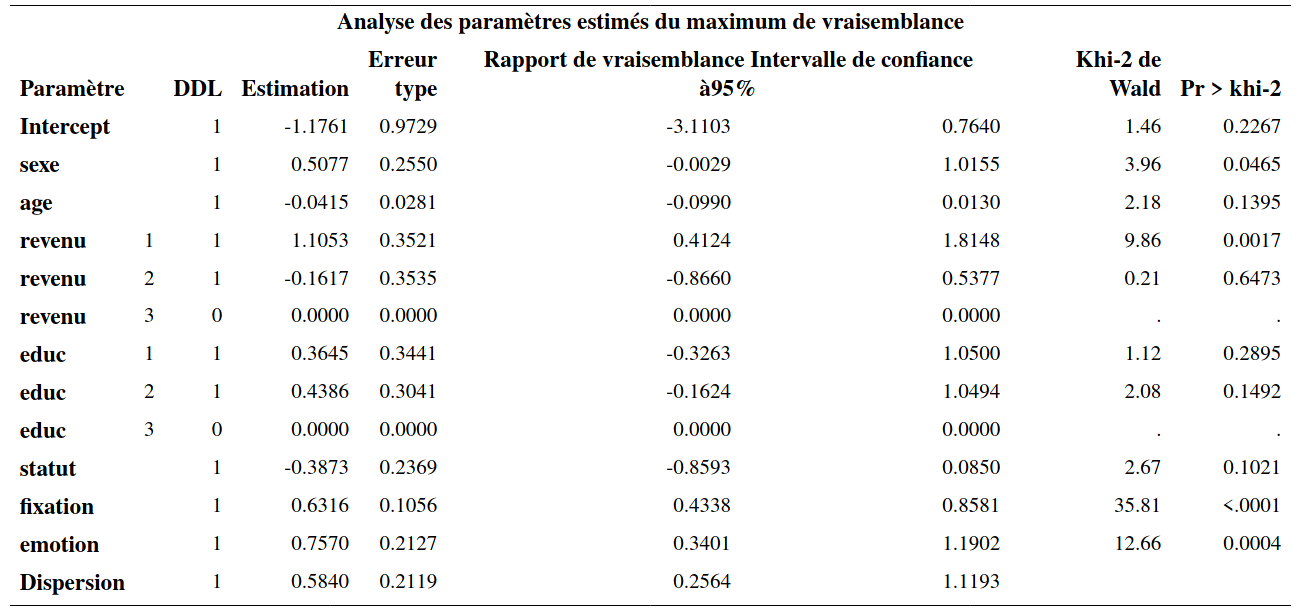
\includegraphics[width = 0.99\linewidth]{img/c4/diapos8-e8}
\end{center}
{\footnotesize 
L'estimé du paramètre d'échelle $\hat{k} = 0.584$. À noter que les intervalles de confiance sont basés sur des rapports de vraisemblance et que leurs conclusions peuvent être différentes de celles tirées à l'aide des valeurs-$p$ du test de Wald; préférer les premières, qui sont plus fiables.


}
\end{frame}

\begin{frame}[fragile]
\frametitle{Sélection de modèles}
\bi
\item Le quotient déviance sur degrés de libertés est plus près de un, mais cette comparaison est informelle.
\item On pourrait utiliser les critères d'information pour choisir le modèle (le plus petit, le mieux); la régression binomiale négative est préférable selon le $\mathsf{AIC}$ et le $\mathsf{BIC}$.
\ei
\begin{center}
\begin{tabular}{crr}
\toprule
 modèle & \multicolumn{1}{c}{Poisson} & \multicolumn{1}{c}{binom. nég.}
 \\ \midrule
$\mathsf{AIC}$ & $392.33$ & $371.25$ \\
 $\mathsf{BIC}$& $420.20$ & $301.91$ \\\bottomrule
\end{tabular}
\end{center}


\end{frame}

\begin{frame}[fragile]
\frametitle{Loi négative binomiale et Poisson}
\bi

\item Quand $k$ tend vers zéro, la loi négative binomiale devient une loi de Poisson. 
\item On peut comparer les deux modèles à l'aide d'un test du rapport de vraisemblance (modèles emboîtés). 
\item  On teste les hypothèses $\Hy_0: k=0, \Hy_1: k\neq 0$ à l'aide de la statistique du rapport de vraisemblance
\bi \item attention! la loi nulle est \textbf{irrégulière} parce que $k$ doit être positif;  quand $n \to \infty$,  il y a une probabilité de $0,5$ que la déviance soit exactement égale à zéro et $0,5$ qu'elle suive une loi $\chi^2_1$ sous $\Hy_0$.
\ei
\item La loi nulle asymptotique est
\begin{align*}
2\{\ell_{\mathsf{negbin}}(\hat{\mu}_{\mathsf{negbin}}, \hat{k}) - \ell_{\mathsf{pois}}(\hat{\mu}_{\mathsf{pois}})\} \stackrel{\cdot}{\sim} \frac{1}{2}\chi^2_1 + \frac{1}{2} \delta_0;
\end{align*}
En pratique: si on a pas $\hat{k}=0$, on calcule la valeur-$p$ comme d'ordinaire à partir de la loi $\chi^2_1$  et on \textbf{divise par deux} la valeur-$p$ pour obtenir la \textbf{valeur correcte}.
\ei
\end{frame}
\begin{frame}[fragile]
\frametitle{Test du rapport de vraisemblance (irrégulier)}
Pour faire les calculs à la main à l'aide des sorties.

\bi \item La ``\textbf{Log-vraisemblance complète}'' donne la valeur de la log-vraisemblance du modèle ajusté, $-174,6250$ pour la régresion binomiale négative et $-186,1639$ pour la régression de Poisson.
\item La différence est $11,5389$ et la statistique du rapport de vraisemblance $23,08$.
\ei

\end{frame}
\begin{frame}[fragile]
\frametitle{Test du rapport de vraisemblance (irrégulier)}
\begin{tcolorbox}[colback=white, colframe=hecblue, title=Code SAS pour le test du rapport de vraisemblance (irrégulier)]
{\small 
\begin{verbatim}
data valp;
valp=(1 - cdf('chisq', 23.08, 1))/2;
run;
proc print data=valp;
run;
\end{verbatim}
}
\end{tcolorbox}
\bi \item La probabilité qu'une loi  $\chi^2_1$ soit plus grande que  $23,08$ est $1.55 \times 10^{-7}$.
\item Puisque le problème est irrégulier, on divise cette probabilité par deux et notre valeur-$p$ est $7.7 \times 10^{-8}$: le modèle de régression binomiale négative est préférable au modèle Poisson.
\ei
\end{frame}

\end{document}
